\section{Pre-emptive Loading}

Another feature of HTTP/2 is that responses can be sent before a corresponding request is received. On a typical website, the HTML file that the browser initially receives will contain a number of other resources (images, code to style the page, advertising) that also need to be requested before the page can be fully displayed. Assuming that all these other request can be done in parallel, this means that the time taken for the page to load is effectively twice that of the time taken to complete a single request.

\begin{figure}
	\centering
	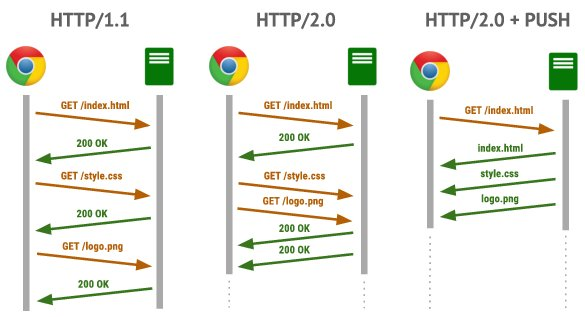
\includegraphics[width=0.8\textwidth]{h2push.jpg}
	\caption{HTTP/2 server push saves round trips from the client to the server.}
	\label{fig:h2push}
\end{figure}

Using HTTP/1.1, many websites avoided this problem by embedding the secondary resources inside the primary HTML file (known as `inlining'), so that the browser does not need to make a second full request to get the extra resources. However HTTP/2 has a feature called `server push' which allows a server to pre-emptively send the secondary resources at the same time as the primary resource, before having received the request for them. So for example on a HTML file that contained two images, upon receiving the request for that HTML file, the server would send both the HTML file and then the two images all at the same time\footnote{The server operator would need to configure beforehand which secondary resources should be sent for a given primary resource.}, avoiding the time needed for the client to receive the response and dispatch another two requests for the images. The behaviour of HTTP/1.1 without inlining, HTTP/2 without server push, and HTTP/2 with server push is shown in figure~\ref{fig:h2push}.

For the web developer, this means that inlining is in theory no longer necessary, as server push achieves much the same function. Additionally server push is more `cache friendly'. Browsers typically cache (meaning save locally) resources that they receive so that they are able to retrieve the file from the local cache instead of having to make another network request\footnote{This is why pages load so fast when you press the back button in a browser}. With server push, a server could in theory remember that a client has image $X$ cached but not image $Y$, and send only image $Y$ in the pre-emptive push. This is superior to inlining where both $X$ and $Y$ would get sent despite $X$ being in the cache, using up unnecessary bandwidth. Additionally, some resources (like the results from a search engine) are dynamically generated and cannot realistically be inlined~\cite{cache-docs}. However with server push, the performance benefits are retained since the server can send the resource as it would any other. Overall, server push provides major benefits since it not only takes off some of the burden of optimising the web page from the designer, but also improves performance in the case where optimisation has been applied.

Unfortunately in practice it is difficult for servers to determine which resources the client currently has cached, and realistically not that many resources are cacheable. This means that if applied incorrectly, server push can even be detrimental to performance as the server can push resources that are already in the browser's cache, wasting unnecessary bandwidth~\cite{push-study}. For this reason, HTTP/2 server push support is not used by many servers (even though all major browsers support it~\cite{server-push}). In a study of 5.32 million HTTP/2 enabled websites, only 595 supported server push on their landing page~\cite{push-study}. It seems that server push will remain largely unused in the future, although there is an extension to HTTP/2~\cite{cache-digest}~being introduced that allows for the client to more effectively inform the server which resources are cached, so that the server does not unnecessarily push already cached resources.

For this reason I have chosen not to implement server push in my web server, but you can find a demonstration at~\cite{push-demo}.
